\chapter{Simulação Numérica e Planejamento de Trajetórias}
\label{cap:simulacao}

Este capítulo descreve a camada de simulação numérica do \textit{Hephaestus}, implementada na classe \texttt{RobotSimulator} do módulo \texttt{simulator.py}. Enquanto o Capítulo~\ref{cap:modelagem} tratou da derivação simbólica e da compilação das equações de movimento, este capítulo aborda como essas equações são integradas numericamente em malha fechada para rastrear trajetórias cartesianas com controle dinâmico de alta fidelidade. As contribuições técnicas centrais deste capítulo compreendem: o planejamento de trajetórias com polinômio cúbico no espaço cartesiano (segmentos lineares e arcos circulares); a extensão do algoritmo CLIK para controle de orientação no espaço de tarefa 6D; a inicialização robusta de postura por Levenberg-Marquardt com busca em linha; o integrador simplético com \textit{substeps} independentes; quatro estratégias de controle não-linear comparáveis em uma única interface; e modelos de forças dissipativas para atrito nas juntas e arrasto hidrodinâmico.

% ==============================================================================
\section{Arquitetura do Simulador}
\label{sec:arq_simulador}
% ==============================================================================

A classe \texttt{RobotSimulator} recebe como entrada um objeto \texttt{RobotMathEngine} (ou \texttt{RobotMathHydro}) previamente processado e realiza, em seu construtor, a compilação de todas as expressões simbólicas em funções numéricas. Conforme descrito na Seção~\ref{sec:lambdify_cse} do Capítulo~\ref{cap:modelagem}, essa compilação é realizada por \texttt{sp.lambdify()} com CSE ativo, produzindo as funções \texttt{func\_M}, \texttt{func\_C}, \texttt{func\_G}, \texttt{func\_J} e o vetor \texttt{funcs\_fk\_all\_links}, que avalia a posição cartesiana de cada elo para a visualização animada \cite{meurer2017sympy}.

A interface pública principal é o método \texttt{run()}, cuja assinatura unifica os parâmetros de configuração da trajetória, do controlador, do integrador e das forças dissipativas em um único ponto de entrada. Internamente, o método \texttt{run()} organiza a simulação em quatro fases:

\begin{enumerate}
    \item \textbf{Inicialização da Postura}: a posição cartesiana inicial $P_i$ é passada ao Levenberg-Marquardt (\texttt{solve\_ik\_initial}) para convergir a uma configuração de juntas $q_0$ compatível antes do início da trajetória.
    \item \textbf{Loop de Integração}: a cada passo visual $\Delta t_{\text{vis}}$, são executados $N_s$ \textit{substeps} físicos $\Delta t_{\text{phys}} = \Delta t_{\text{vis}} / N_s$, cada um compreendendo: planejamento de trajetória, CLIK, avaliação de $M$, $C$, $G$, cálculo do torque de controle, aplicação das forças dissipativas e integração simplética.
    \item \textbf{Coleta de Resultados}: ao final de cada passo visual, os erros de junta $e = q_d - q$, os torques aplicados $\tau$ e os dados de animação (posições FK de todos os elos e matrizes de rotação) são armazenados.
    \item \textbf{Retorno}: o método retorna as séries temporais $\{t_i, e_i, \tau_i\}$ e a lista de frames de animação, que são consumidos pela interface gráfica para plotagem e renderização interativa.
\end{enumerate}

A detecção automática da fronteira veículo/braço — pela contagem das juntas iniciais sem vetor de elo estrutural nulo — permite que o simulador opere tanto em manipuladores terrestres puros quanto em UVMSs, compilando separadamente a matriz de rotação do frame do veículo (\texttt{func\_R\_vehicle}) para visualização da orientação do corpo base \cite{antonelli2014modelling, fossen2011handbook}. As Figuras~\ref{fig:loop_init} e~\ref{fig:loop_controle} detalham o fluxo interno do método \texttt{run()}: a fase de inicialização (Figura~\ref{fig:loop_init}) e o passo de controle repetido a cada substep físico (Figura~\ref{fig:loop_controle}).

\begin{figure}[htbp]
    \centering
    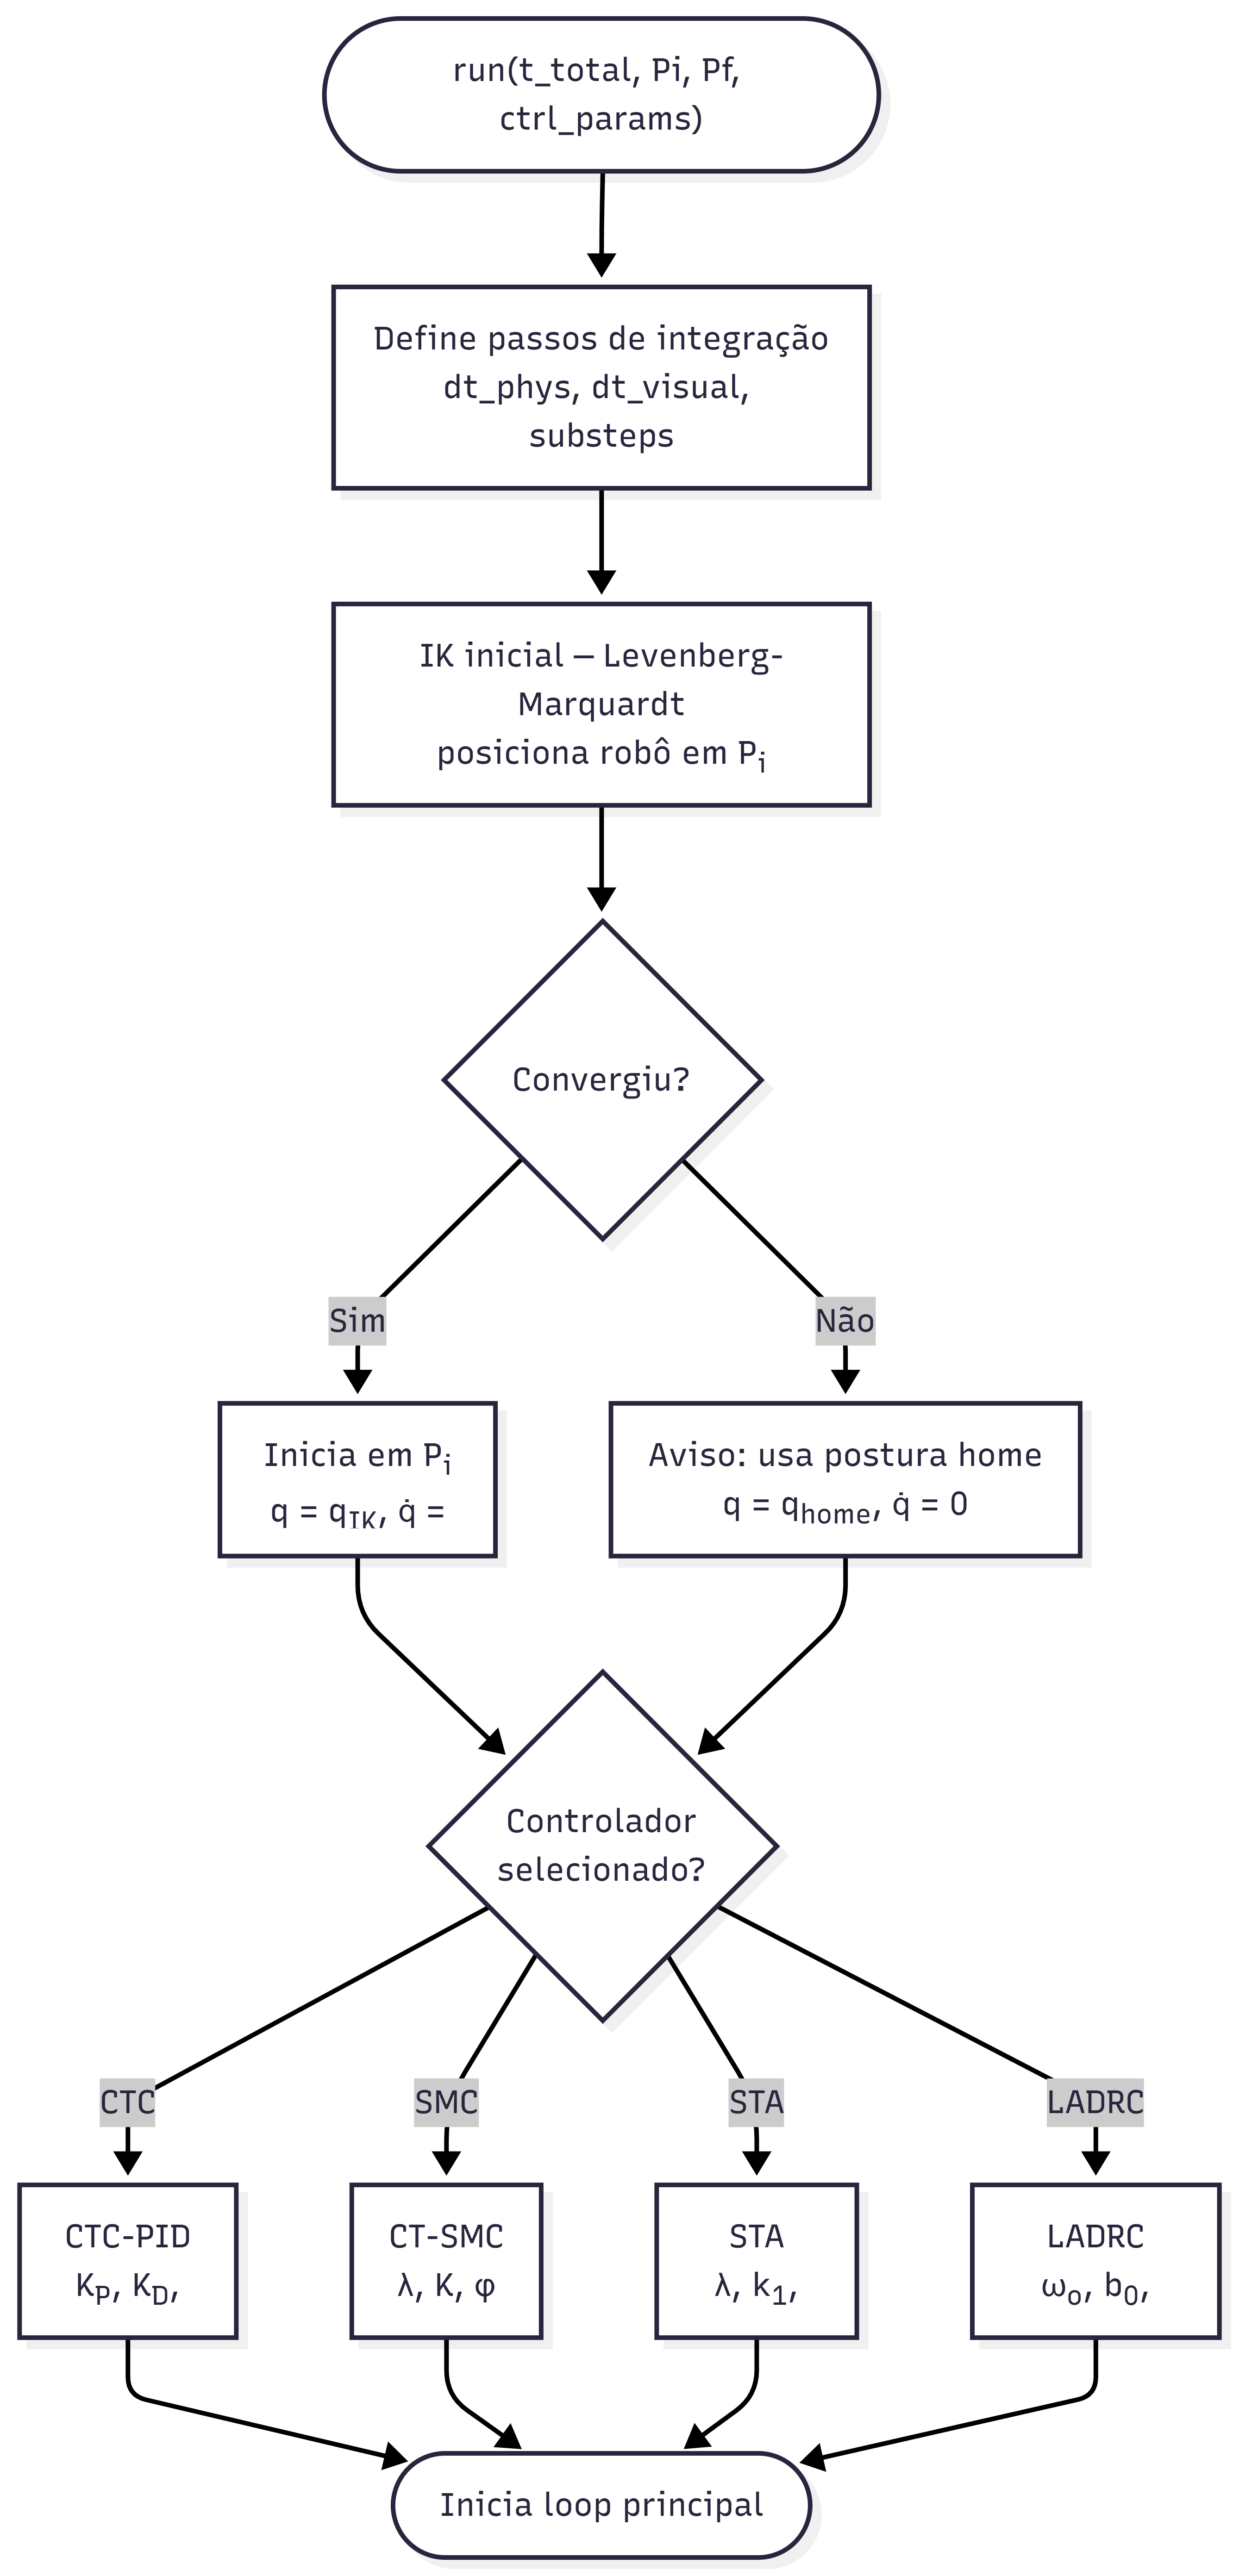
\includegraphics[width=0.65\textwidth]{figuras/Diagramas/Diagrama 7a — Loop de Simulação Inicialização.png}
    \caption{Fase de inicialização do simulador: resolução da IK estática por Levenberg-Marquardt com busca em linha (Seção~\ref{sec:ik_initial}), configuração do controlador e do executor paralelo, e verificação das condições de estabilidade numérica (Seção~\ref{sec:estabilidade_num}).}
    \label{fig:loop_init}
\end{figure}

\begin{figure}[htbp]
    \centering
    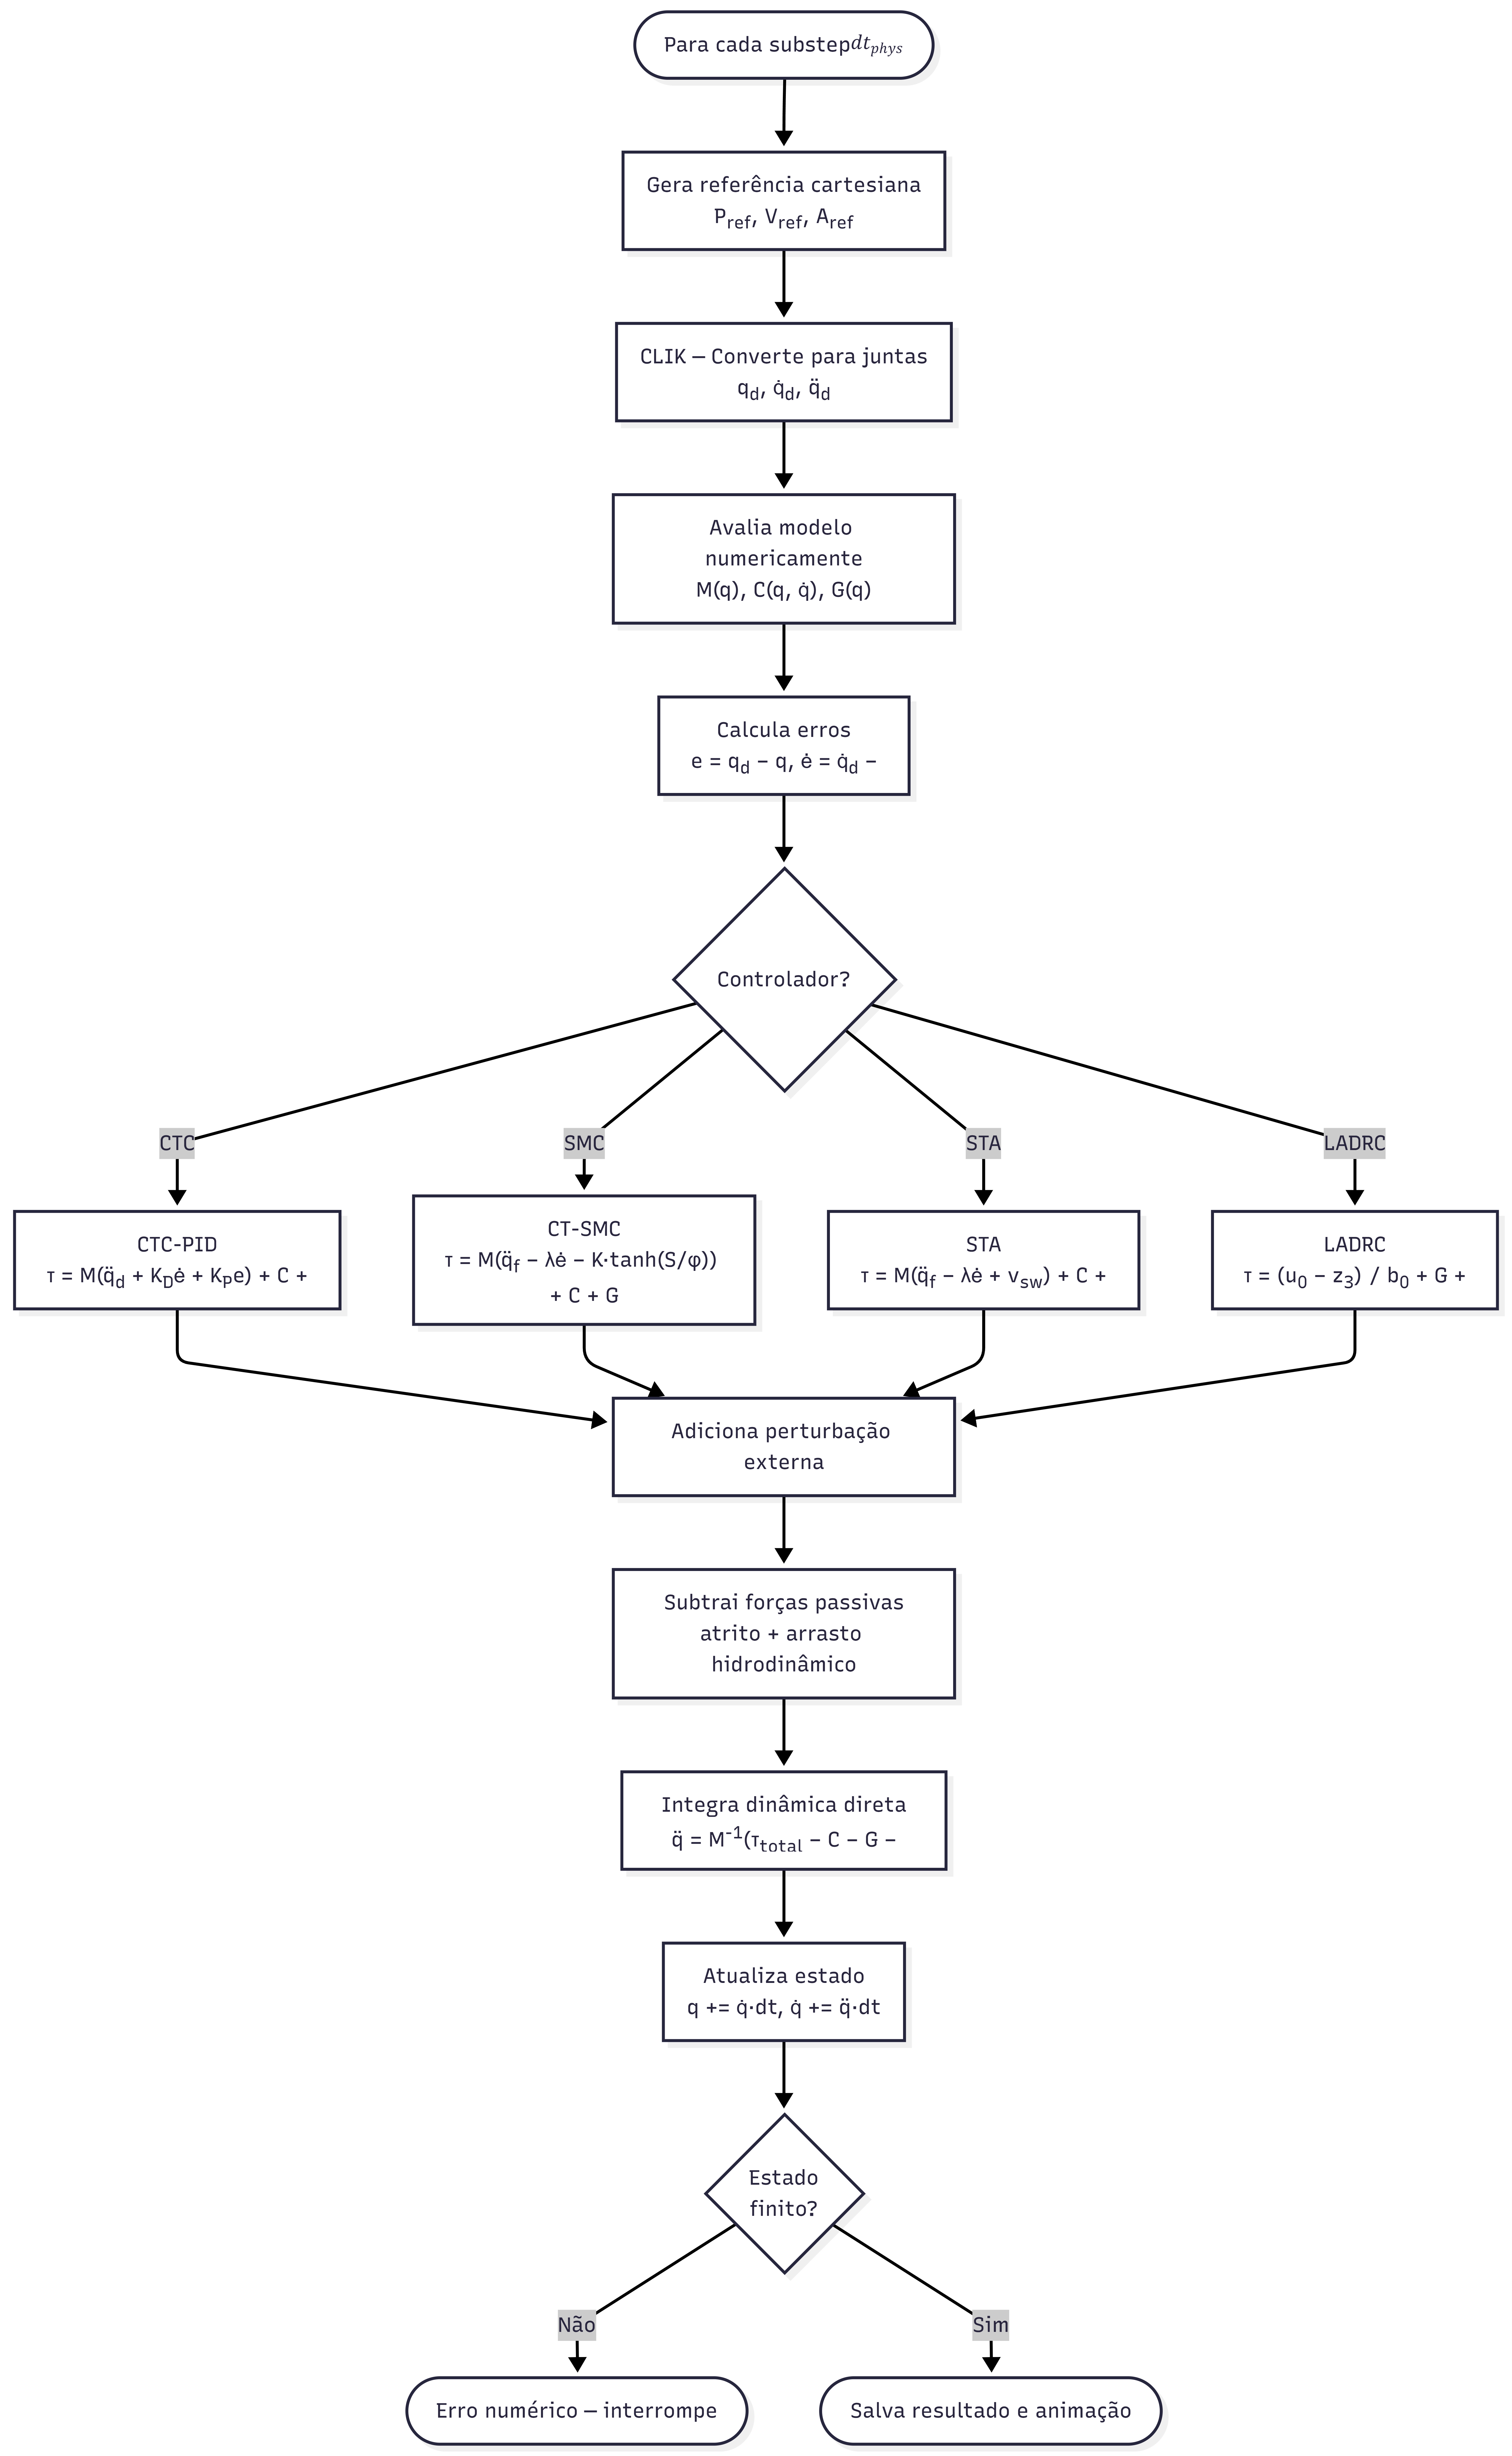
\includegraphics[width=0.88\textwidth]{figuras/Diagramas/Diagrama 7b — Loop de Simulação Passo de Controle.png}
    \caption{Passo de controle físico executado a cada substep $\Delta t_{\text{phys}}$: planejamento de trajetória, CLIK 6D, avaliação paralela de $M$, $C$, $G$, cálculo do torque de controle, aplicação das forças dissipativas e integração simplética de Euler (Equações~\eqref{eq:symplectic1}--\eqref{eq:symplectic2}).}
    \label{fig:loop_controle}
\end{figure}

% ==============================================================================
\section{Planejamento de Trajetórias no Espaço Cartesiano}
\label{sec:traj_planning}
% ==============================================================================

O planejamento de trajetórias define as referências de posição $P_{\text{ref}}(t)$, velocidade $\dot{P}_{\text{ref}}(t)$ e aceleração $\ddot{P}_{\text{ref}}(t)$ que o efetuador deve rastrear ao longo do tempo. Siciliano et al. \cite{siciliano2009robotics} e Craig \cite{craig1989introduction} distinguem o planejamento no espaço de juntas do planejamento no espaço cartesiano; este trabalho adota o segundo, em que as referências são geradas diretamente na posição do efetuador e convertidas para comandos de junta pelo CLIK a cada instante.

\subsection{Polinômio Cúbico de Interpolação}

Toda trajetória implementada no \textit{Hephaestus} utiliza o parâmetro de tempo normalizado $\tau = t / T \in [0,1]$, onde $T$ é a duração total do segmento, interpolado pelo polinômio cúbico:
\begin{equation}
    s(\tau) = 3\tau^2 - 2\tau^3,
    \label{eq:cubic_s}
\end{equation}
com derivadas:
\begin{equation}
    \dot{s} = \frac{6\tau - 6\tau^2}{T}, \qquad
    \ddot{s} = \frac{6 - 12\tau}{T^2}.
    \label{eq:cubic_ds}
\end{equation}

Este perfil garante $s(0) = 0$, $s(1) = 1$, $\dot{s}(0) = \dot{s}(1) = 0$ — ou seja, partida e parada suaves — e aceleração máxima $|\ddot{s}|_{\max} = 6/T^2$ no instante $T/2$ \cite{siciliano2009robotics}. A continuidade da velocidade nos extremos é essencial para evitar descontinuidades no sinal de referência do CLIK que seriam amplificadas pelos ganhos derivativos do controlador \cite{craig1989introduction}. O polinômio de grau 5 (que garantiria continuidade de aceleração nos extremos) não foi adotado por apresentar pico de aceleração levemente superior para o mesmo tempo de trajetória, conforme análise comparativa de Siciliano et al. \cite{siciliano2009robotics}.

\subsection{Segmento de Reta}

Para a trajetória linear de $P_i$ a $P_f$, a referência cartesiana é:
\begin{align}
    P_{\text{ref}}(t) &= P_i + (P_f - P_i)\,s(\tau), \label{eq:traj_line_P}\\
    \dot{P}_{\text{ref}}(t) &= (P_f - P_i)\,\dot{s}(\tau), \label{eq:traj_line_V}\\
    \ddot{P}_{\text{ref}}(t) &= (P_f - P_i)\,\ddot{s}(\tau). \label{eq:traj_line_A}
\end{align}

A disponibilidade explícita de $\dot{P}_{\text{ref}}$ e $\ddot{P}_{\text{ref}}$ é fundamental para o \textit{feedforward} de velocidade e aceleração no CLIK, que reduz o erro de rastreamento em regime dinâmico em comparação com o uso exclusivo de realimentação proporcional de posição \cite{chiaverini1994review, siciliano2009robotics}.

\subsection{Arco Circular}

A trajetória circular é parametrizada pelo centro $C$, dois vetores ortonormais $e_1$, $e_2$ no plano do arco, raio $R$, ângulo inicial $\theta_0$ e ângulo final $\theta_f$. O centro é determinado geometricamente como o ponto equidistante de $P_i$ e $P_f$ ao longo da direção perpendicular à corda $v = P_f - P_i$ no plano definido pelo vetor normal $\hat{n}$:
\begin{equation}
    C = \frac{P_i + P_f}{2} \pm h\,\frac{(P_f - P_i) \times \hat{n}}{\|(P_f - P_i) \times \hat{n}\|}, \qquad
    h = \sqrt{R^2 - \frac{\|P_f - P_i\|^2}{4}},
    \label{eq:circle_center}
\end{equation}
com sinal determinado pelo parâmetro de sentido de percurso. A trajetória é então:
\begin{equation}
    P(t) = C + R\left[\cos(\theta(t))\,e_1 + \sin(\theta(t))\,e_2\right], \quad
    \theta(t) = \theta_0 + (\theta_f - \theta_0)\,s(\tau),
    \label{eq:circle_traj}
\end{equation}
com velocidade e aceleração obtidas por diferenciação analítica:
\begin{align}
    \dot{P}(t) &= R\,\dot{\theta}\,\left[-\sin(\theta)\,e_1 + \cos(\theta)\,e_2\right], \label{eq:circle_V}\\
    \ddot{P}(t) &= R\,\left[\ddot{\theta}\,\hat{t}(\theta) + \dot{\theta}^2\,\hat{n}(\theta)\right],
    \label{eq:circle_A}
\end{align}
onde $\hat{t} = -\sin(\theta)\,e_1 + \cos(\theta)\,e_2$ é o vetor tangente e $\hat{n} = -\cos(\theta)\,e_1 - \sin(\theta)\,e_2$ é o vetor normal centrípeto. A componente centrípeta $\dot{\theta}^2\,\hat{n}$ da aceleração é frequentemente omitida em abordagens simplificadas, mas sua inclusão é necessária para que o \textit{feedforward} de aceleração no CLIK seja fisicamente correto em trajetórias circulares de alta velocidade \cite{siciliano2009robotics}.

Uma verificação de segurança automática é aplicada: se a distância entre $P_i$ e $P_f$ excede o diâmetro $2R$, o raio é automaticamente estendido para $R = \|P_f - P_i\|/2 + \varepsilon$, garantindo geometria factível. Caso o vetor $(P_f - P_i) \times \hat{n}$ seja nulo (pontos colineares com a normal), a trajetória degrada graciosamente para um segmento de reta \cite{siciliano2009robotics}. A Figura~\ref{fig:traj_planning} apresenta o fluxo de geração das referências de posição, velocidade e aceleração para os dois tipos de trajetória implementados e a integração com o polinômio cúbico.

\begin{figure}[htbp]
    \centering
    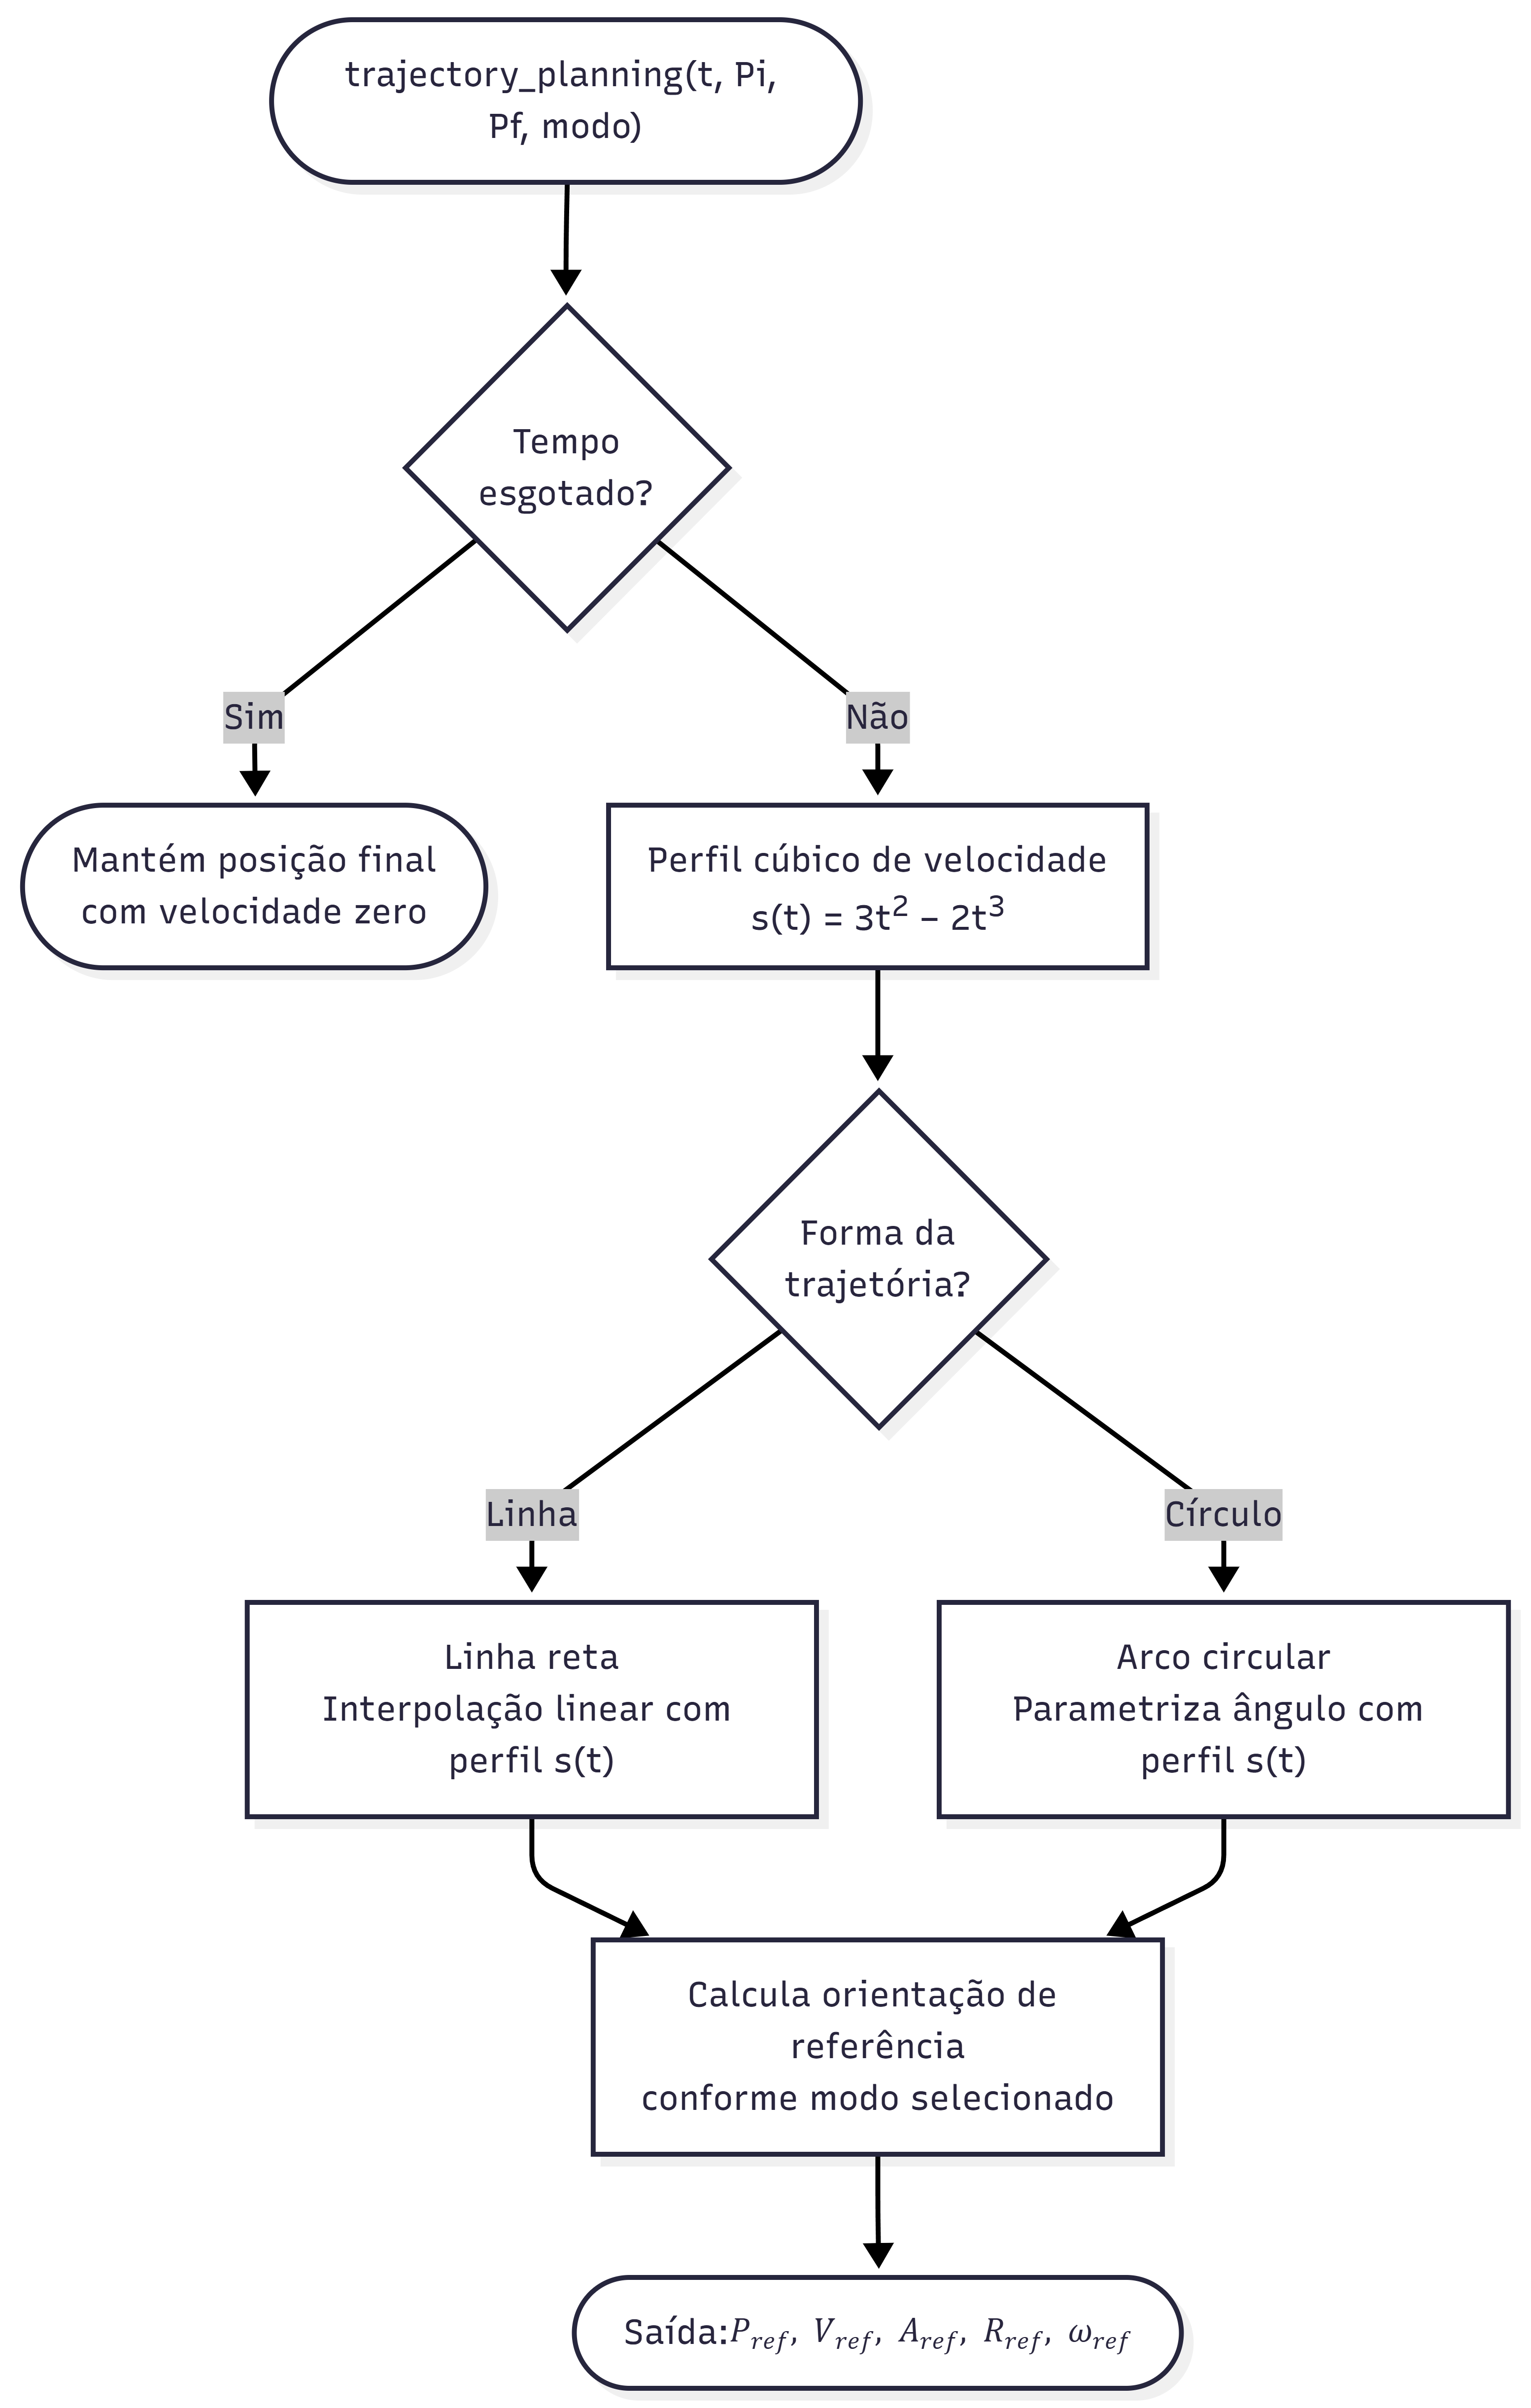
\includegraphics[width=0.90\textwidth]{figuras/Diagramas/Diagrama 5 — Planejamento de Trajetória.png}
    \caption{Fluxo de planejamento de trajetória no espaço cartesiano: o parâmetro cúbico $s(\tau)$ (Equação~\eqref{eq:cubic_s}) é aplicado ao segmento de reta (Equações~\eqref{eq:traj_line_P}--\eqref{eq:traj_line_A}) ou ao arco circular (Equações~\eqref{eq:circle_traj}--\eqref{eq:circle_A}), gerando triplas $\{P_{\text{ref}}, \dot{P}_{\text{ref}}, \ddot{P}_{\text{ref}}\}$ a cada passo de integração para o CLIK \cite{siciliano2009robotics, craig1989introduction}.}
    \label{fig:traj_planning}
\end{figure}

\subsection{Modos de Referência de Orientação}
\label{sec:orient_modes}

O \textit{Hephaestus} suporta seis modos distintos de referência de orientação do efetuador, selecionáveis independentemente do tipo de trajetória posicional:

\begin{enumerate}
    \item \textbf{Livre} (\textit{orientation-free}): nenhuma restrição de orientação é imposta; o CLIK opera apenas com o Jacobiano posicional $3 \times N$. Este modo é o padrão e adequado para tarefas de posicionamento puro.
    
    \item \textbf{Fixa}: a orientação é mantida constante e igual à rotação $R_0$ capturada na postura inicial. Implementado como $R_{\text{ref}}(t) = R_0$, $\omega_{\text{ref}} = 0$. Útil para tarefas de transporte com efetuador estabilizado \cite{siciliano2009robotics}.
    
    \item \textbf{Tangente à Trajetória}: o eixo $z$ do efetuador é alinhado à tangente instantânea da trajetória:
    \begin{equation}
        \hat{z}(t) = \frac{\dot{P}_{\text{ref}}(t)}{\|\dot{P}_{\text{ref}}(t)\|}, \qquad
        \omega_{\text{ref}} = \hat{z} \times \dot{\hat{z}},
        \label{eq:orient_tangent}
    \end{equation}
    onde $\dot{\hat{z}}$ é obtido por diferenciação analítica de $\hat{z}$ em relação ao tempo. Empregado em tarefas de corte, pintura ou inspeção ao longo da trajetória \cite{siciliano2009robotics}.
    
    \item \textbf{Apontar para o Alvo}: o eixo $z$ do efetuador é continuamente orientado em direção ao ponto $P_f$:
    \begin{equation}
        \hat{z}(t) = \frac{P_f - P_{\text{ref}}(t)}{\|P_f - P_{\text{ref}}(t)\|}, \qquad
        \omega_{\text{ref}} = \hat{z} \times \left[\frac{-\dot{P}_{\text{ref}}}{\|P_f - P_{\text{ref}}\|} - \frac{(P_f - P_{\text{ref}}) \cdot (-\dot{P}_{\text{ref}})}{\|P_f - P_{\text{ref}}\|^3}(P_f - P_{\text{ref}})\right].
        \label{eq:orient_point}
    \end{equation}
    Adequado para tarefas de solda, furação ou interação com um alvo fixo \cite{chiaverini1997singularity}.
    
    \item \textbf{SLERP} (\textit{Spherical Linear Interpolation}): interpola suavemente a orientação entre $R_0$ (postura inicial) e $R_f$ (orientação final desejada) ao longo do geodésico em $SO(3)$:
    \begin{equation}
        R_{\text{ref}}(t) = R_0 \left(R_0^\top R_f\right)^{s(\tau)}, \qquad
        \omega_{\text{ref}} = \dot{s}\,\theta_{\text{total}}\,R_0\,\hat{a}_{\text{local}},
        \label{eq:slerp_impl}
    \end{equation}
    onde $\theta_{\text{total}}$ é o ângulo total de rotação e $\hat{a}_{\text{local}}$ é o eixo de rotação no referencial de $R_0$, extraído pela decomposição eixo-ângulo de $R_0^\top R_f$ \cite{shoemake1985animating, dam1998quaternions}. A velocidade angular de referência $\omega_{\text{ref}}$ garante que o \textit{feedforward} rotacional seja fisicamente correto, não apenas proporcional ao erro.
    
    \item \textbf{Normal à Superfície}: o eixo $z$ é mantido alinhado a um vetor normal fixo $\hat{n}$ fornecido pelo usuário, com $\omega_{\text{ref}} = 0$. Adequado para tarefas de usinagem ou inspeção perpendicular a superfícies planas \cite{siciliano2009robotics}.
\end{enumerate}

Os modos 2 a 6 ativam o Jacobiano completo $6 \times N$ no CLIK, descrito na Seção~\ref{sec:clik_6d}, combinando controle de posição e orientação no mesmo algoritmo. A Figura~\ref{fig:modos_orientacao} compara os seis modos de referência de orientação implementados, indicando o sinal de referência gerado por cada um e os casos de uso típicos.

\begin{figure}[htbp]
    \centering
    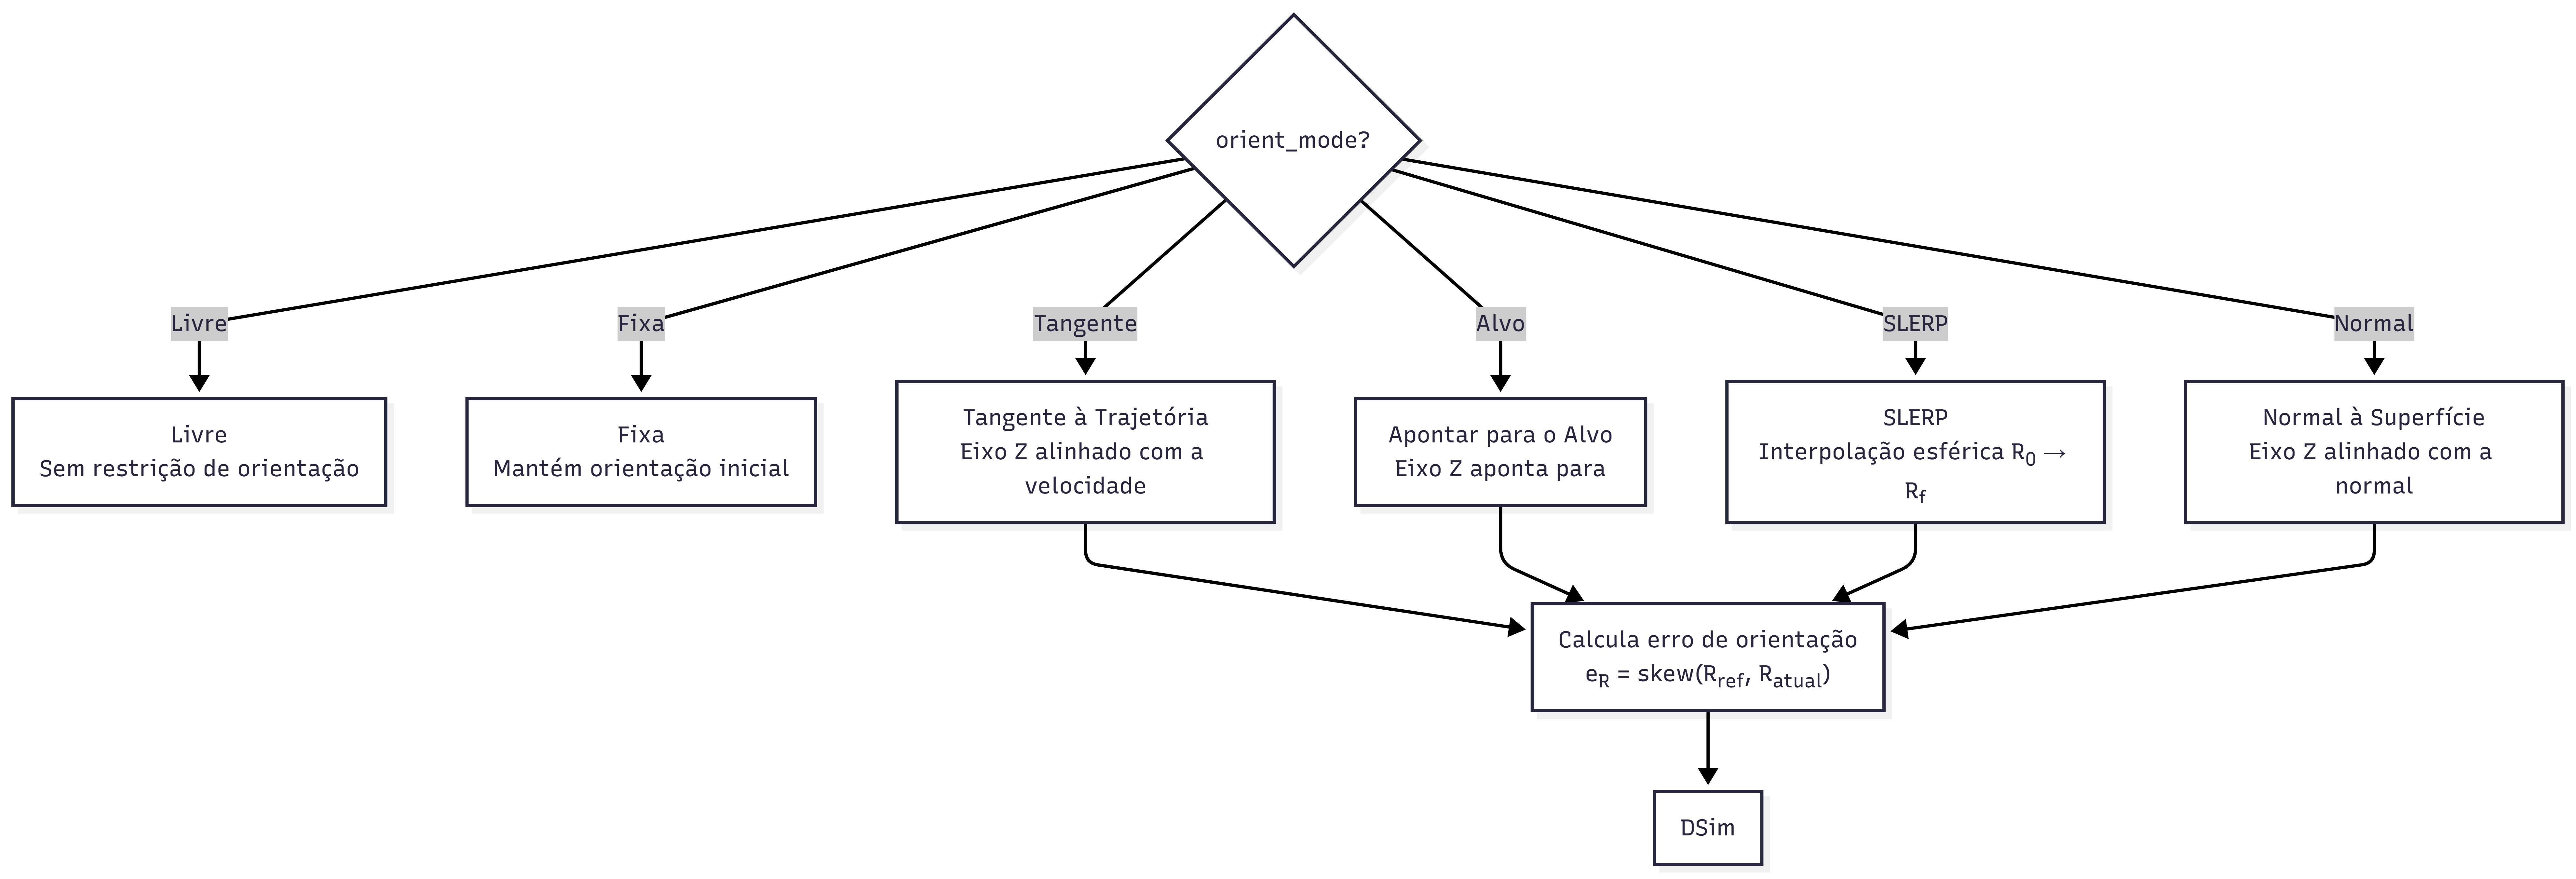
\includegraphics[width=0.9\textwidth]{figuras/Diagramas/Diagrama 6b — Modos de Orientação do Efetuador.png}
    \caption{Modos de referência de orientação do efetuador disponíveis no \textit{Hephaestus}: Livre (apenas controle posicional), Fixa, Tangente à Trajetória, Apontar para o Alvo, SLERP geodésico \cite{shoemake1985animating} e Normal à Superfície. Os modos 2--6 ativam o Jacobiano completo $J \in \mathbb{R}^{6 \times N}$ e o erro de orientação da Equação~\eqref{eq:orient_error_impl}.}
    \label{fig:modos_orientacao}
\end{figure}

% ==============================================================================
\section{Inicialização da Postura: Levenberg-Marquardt com Busca em Linha}
\label{sec:ik_initial}
% ==============================================================================

Antes do início da trajetória, o \textit{Hephaestus} resolve o problema de IK estática para posicionar o efetuador em $P_i$ a partir da postura inicial $q_0$ (postura \textit{home} ou última postura convergida). Para garantir convergência robusta mesmo próximo de singularidades ou partindo de configurações distantes, é empregada uma variante do algoritmo de Levenberg-Marquardt \cite{marquardt1963algorithm, more2006levenberg} com busca em linha por \textit{backtracking} (regra de Armijo \cite{armijo1966minimization}).

O algoritmo iterativo é descrito a seguir. A cada iteração $k$:
\begin{enumerate}
    \item Avalia a posição atual $p_k = f_{\text{FK}}(q_k)$ e o erro $e_k = P_i - p_k$.
    \item Se $\|e_k\| < \varepsilon_{\text{tol}}$, termina com convergência.
    \item Calcula o passo DLS:
    \begin{equation}
        \Delta q = J_{\text{pos}}^\top \left(J_{\text{pos}} J_{\text{pos}}^\top + \lambda_k^2 I_3\right)^{-1} e_k,
        \label{eq:lm_step}
    \end{equation}
    onde $J_{\text{pos}} \in \mathbb{R}^{3 \times N}$ é o Jacobiano posicional e $\lambda_k$ é o parâmetro de amortecimento corrente.
    \item Executa busca em linha por \textit{backtracking}: tenta $q_{k+1} = q_k + \alpha \Delta q$ com $\alpha = 1, 0.5, 0.25, \ldots$ até $\|P_i - f_{\text{FK}}(q_{k+1})\| < \|e_k\|$.
    \item Atualiza $\lambda$ adaptativamente: $\lambda \leftarrow 0.9\lambda$ se houve descida (passo aceito), $\lambda \leftarrow 1.5\lambda$ se não houve (passo rejeitado), com limites $\lambda \in [10^{-4},\, 10]$.
    \item Detecta estagnação: se $|\|e_{k-1}\| - \|e_k\|| < 0.1\,\varepsilon_{\text{tol}}$ por 10 iterações consecutivas, interrompe.
\end{enumerate}

A estratégia adaptativa de $\lambda$ é a essência do algoritmo de Levenberg-Marquardt: para erros grandes (longe do mínimo), $\lambda$ grande amortece o passo, comportando-se como o método do gradiente; próximo do mínimo, $\lambda$ pequeno permite convergência quadrática típica de Newton-Gauss \cite{more2006levenberg}. A combinação com a busca em linha de Armijo confere estabilidade adicional quando o Jacobiano é mal-condicionado, conforme demonstrado por Nakamura e Hanafusa \cite{nakamura1986inverse} e Wampler \cite{wampler2007manipulator} para IK de manipuladores com singularidades.

% ==============================================================================
\section{Cinemática Inversa em Malha Fechada (CLIK)}
\label{sec:clik}
% ==============================================================================

\subsection{Formulação do CLIK Posicional (3D)}

Durante a trajetória, a cada passo de integração, o CLIK (Closed-Loop Inverse Kinematics) \cite{samson1991robot, chiaverini1994review} converte a referência cartesiana $\{P_{\text{ref}}, \dot{P}_{\text{ref}}, \ddot{P}_{\text{ref}}\}$ em referências de junta $\{q_d, \dot{q}_d, \ddot{q}_d\}$. A lei de velocidade de junta no modo posicional é:
\begin{equation}
    \dot{q}_d = J_{\text{DLS}}^{\dagger}\left[\dot{P}_{\text{ref}} + K_P\,e_{\text{pos}}\right] + (I - J_{\text{DLS}}^{\dagger} J_{\text{pos}})\,\dot{q}_0,
    \label{eq:clik_pos}
\end{equation}
onde $e_{\text{pos}} = P_{\text{ref}} - p_{\text{curr}}$ é o erro de posição cartesiano, $K_P = K_{p,\text{IK}} \cdot I_3$ é o ganho proporcional do CLIK, e o último termo projeta uma velocidade auxiliar $\dot{q}_0$ no espaço nulo de $J_{\text{pos}}$ para controle de redundância \cite{chiaverini1997singularity, liegeois1977automatic}.

A pseudo-inversa amortecida (DLS) $J_{\text{DLS}}^{\dagger} \in \mathbb{R}^{N \times 3}$ é \cite{nakamura1986inverse, wampler2007manipulator}:
\begin{equation}
    J_{\text{DLS}}^{\dagger} = J_{\text{pos}}^\top \left(J_{\text{pos}} J_{\text{pos}}^\top + \lambda_{\text{DLS}}^2 I_3\right)^{-1}.
    \label{eq:dls_pos}
\end{equation}

A posição de junta de referência é obtida por integração de Euler explícita:
\begin{equation}
    q_d(t + \Delta t) = q_{\text{curr}} + \dot{q}_d\, \Delta t,
    \label{eq:clik_q_int}
\end{equation}
e o termo de aceleração de referência é calculado para \textit{feedforward}:
\begin{equation}
    \ddot{q}_d = J_{\text{DLS}}^{\dagger} \left[\ddot{P}_{\text{ref}} + K_D^{\text{IK}}\,\dot{e}_{\text{vel}} - \dot{J}\dot{q}\right],
    \label{eq:clik_ddq}
\end{equation}
onde $K_D^{\text{IK}} = 2\sqrt{K_P}$ e o termo $\dot{J}\dot{q}$ é a correção de deriva do Jacobiano, calculada por diferença finita de $J_{\text{pos}}$ entre passos consecutivos \cite{siciliano2009robotics}.

\subsection{Limitação de Velocidade de Junta}

Para evitar descontinuidades e prevenir movimentos bruscos próximos de singularidades, a velocidade de junta total $\dot{q}_d$ (incluindo a contribuição do espaço nulo) é saturada suavemente pela função hiperbólica tangente:
\begin{equation}
    \dot{q}_d^{\text{sat}} = \dot{q}_{\text{lim}}\,\tanh\!\left(\frac{\dot{q}_d}{\dot{q}_{\text{lim}}}\right),
    \label{eq:dq_saturation}
\end{equation}
onde $\dot{q}_{\text{lim}}$ é o limite de velocidade por junta. O uso de $\tanh$ em vez de \textit{clipping} linear garante diferenciabilidade e preserva a direção do vetor de velocidade para valores abaixo do limite, o que é importante para a qualidade do \textit{feedforward} \cite{siciliano2009robotics}.

\subsection{Controle de Orientação no Espaço de Tarefa 6D}
\label{sec:clik_6d}

Quando um modo de orientação diferente de \textit{Livre} é selecionado, o CLIK é estendido para o espaço de tarefa 6D, utilizando o Jacobiano completo $J \in \mathbb{R}^{6 \times N}$ e combinando o controle de posição e orientação em uma única lei de velocidade. O erro de orientação é calculado pela formulação de anel (skew-symmetric) \cite{chiaverini1997singularity}:
\begin{equation}
    e_R = \frac{1}{2}\,\text{vee}\!\left(R_{\text{ref}} R_{\text{curr}}^\top - R_{\text{curr}} R_{\text{ref}}^\top\right),
    \label{eq:orient_error_impl}
\end{equation}
onde $R_{\text{curr}}$ é a rotação corrente do efetuador obtida por $\texttt{func\_R\_last}(q, \cdot)$ e $R_{\text{ref}}$ é a rotação de referência do modo selecionado (Seção~\ref{sec:orient_modes}). Esta formulação é proporcional ao vetor eixo-ângulo para erros pequenos e evita singularidades de representação por ângulos de Euler \cite{siciliano2009robotics}.

O vetor de velocidade de tarefa 6D é:
\begin{equation}
    v_{\text{task}} = \begin{bmatrix} \dot{P}_{\text{ref}} + K_P\,e_{\text{pos}} \\ \omega_{\text{ref}} + K_P^{\text{or}}\,e_R \end{bmatrix} \in \mathbb{R}^6,
    \label{eq:task_vel_6d}
\end{equation}
onde $K_P^{\text{or}}$ é o ganho proporcional de orientação e $\omega_{\text{ref}}$ é a velocidade angular de referência fornecida pelo modo de orientação correspondente. A pseudo-inversa amortecida 6D é:
\begin{equation}
    J_{6,\lambda}^{\dagger} = J^\top\left(JJ^\top + \lambda_{\text{DLS}}^2 I_6\right)^{-1} \in \mathbb{R}^{N \times 6},
    \label{eq:dls_6d}
\end{equation}
e a lei de velocidade de junta no modo 6D segue a mesma estrutura da Equação~\eqref{eq:clik_pos}, com $J_{\text{pos}}$ substituído por $J$ e o vetor de erro por $v_{\text{task}}$ \cite{chiaverini1994review, chiaverini1997singularity}. O espaço nulo agora depende de $J_{6,\lambda}^{\dagger} J \in \mathbb{R}^{N \times N}$, e a gestão de redundância via projeção da lei $K_n(q_{\text{home}} - q)$ permanece idêntica \cite{liegeois1977automatic}.

\subsection{Gestão de Redundância via Espaço Nulo}

Para sistemas com $N > 6$ graus de liberdade (ou $N > 3$ no modo posicional), o operador de projeção no espaço nulo $P_n = I - J_\lambda^\dagger J$ define um subespaço de velocidades de junta que não afetam o movimento do efetuador. O \textit{Hephaestus} utiliza esse subespaço para atrair a configuração de junta à postura \textit{home} preferida \cite{chiaverini1997singularity}:
\begin{equation}
    \dot{q}_0 = K_n\,(q_{\text{home}} - q_{\text{curr}}),
    \label{eq:null_space}
\end{equation}
onde $K_n$ é o ganho de espaço nulo (ajustável pelo usuário). Esta abordagem, introduzida por Liegeois \cite{liegeois1977automatic} e consolidada por Chiaverini et al. \cite{chiaverini1997singularity}, garante que o robô tenda à postura de maior manipulabilidade ou com limites de junta mais distantes, melhorando a qualidade do rastreamento ao longo de trajetórias extensas. O fluxo completo do CLIK — incluindo DLS, feedforward de velocidade e aceleração, correção de deriva do Jacobiano e projeção no espaço nulo — é esquematizado na Figura~\ref{fig:clik_cinematica}.

\begin{figure}[htbp]
    \centering
    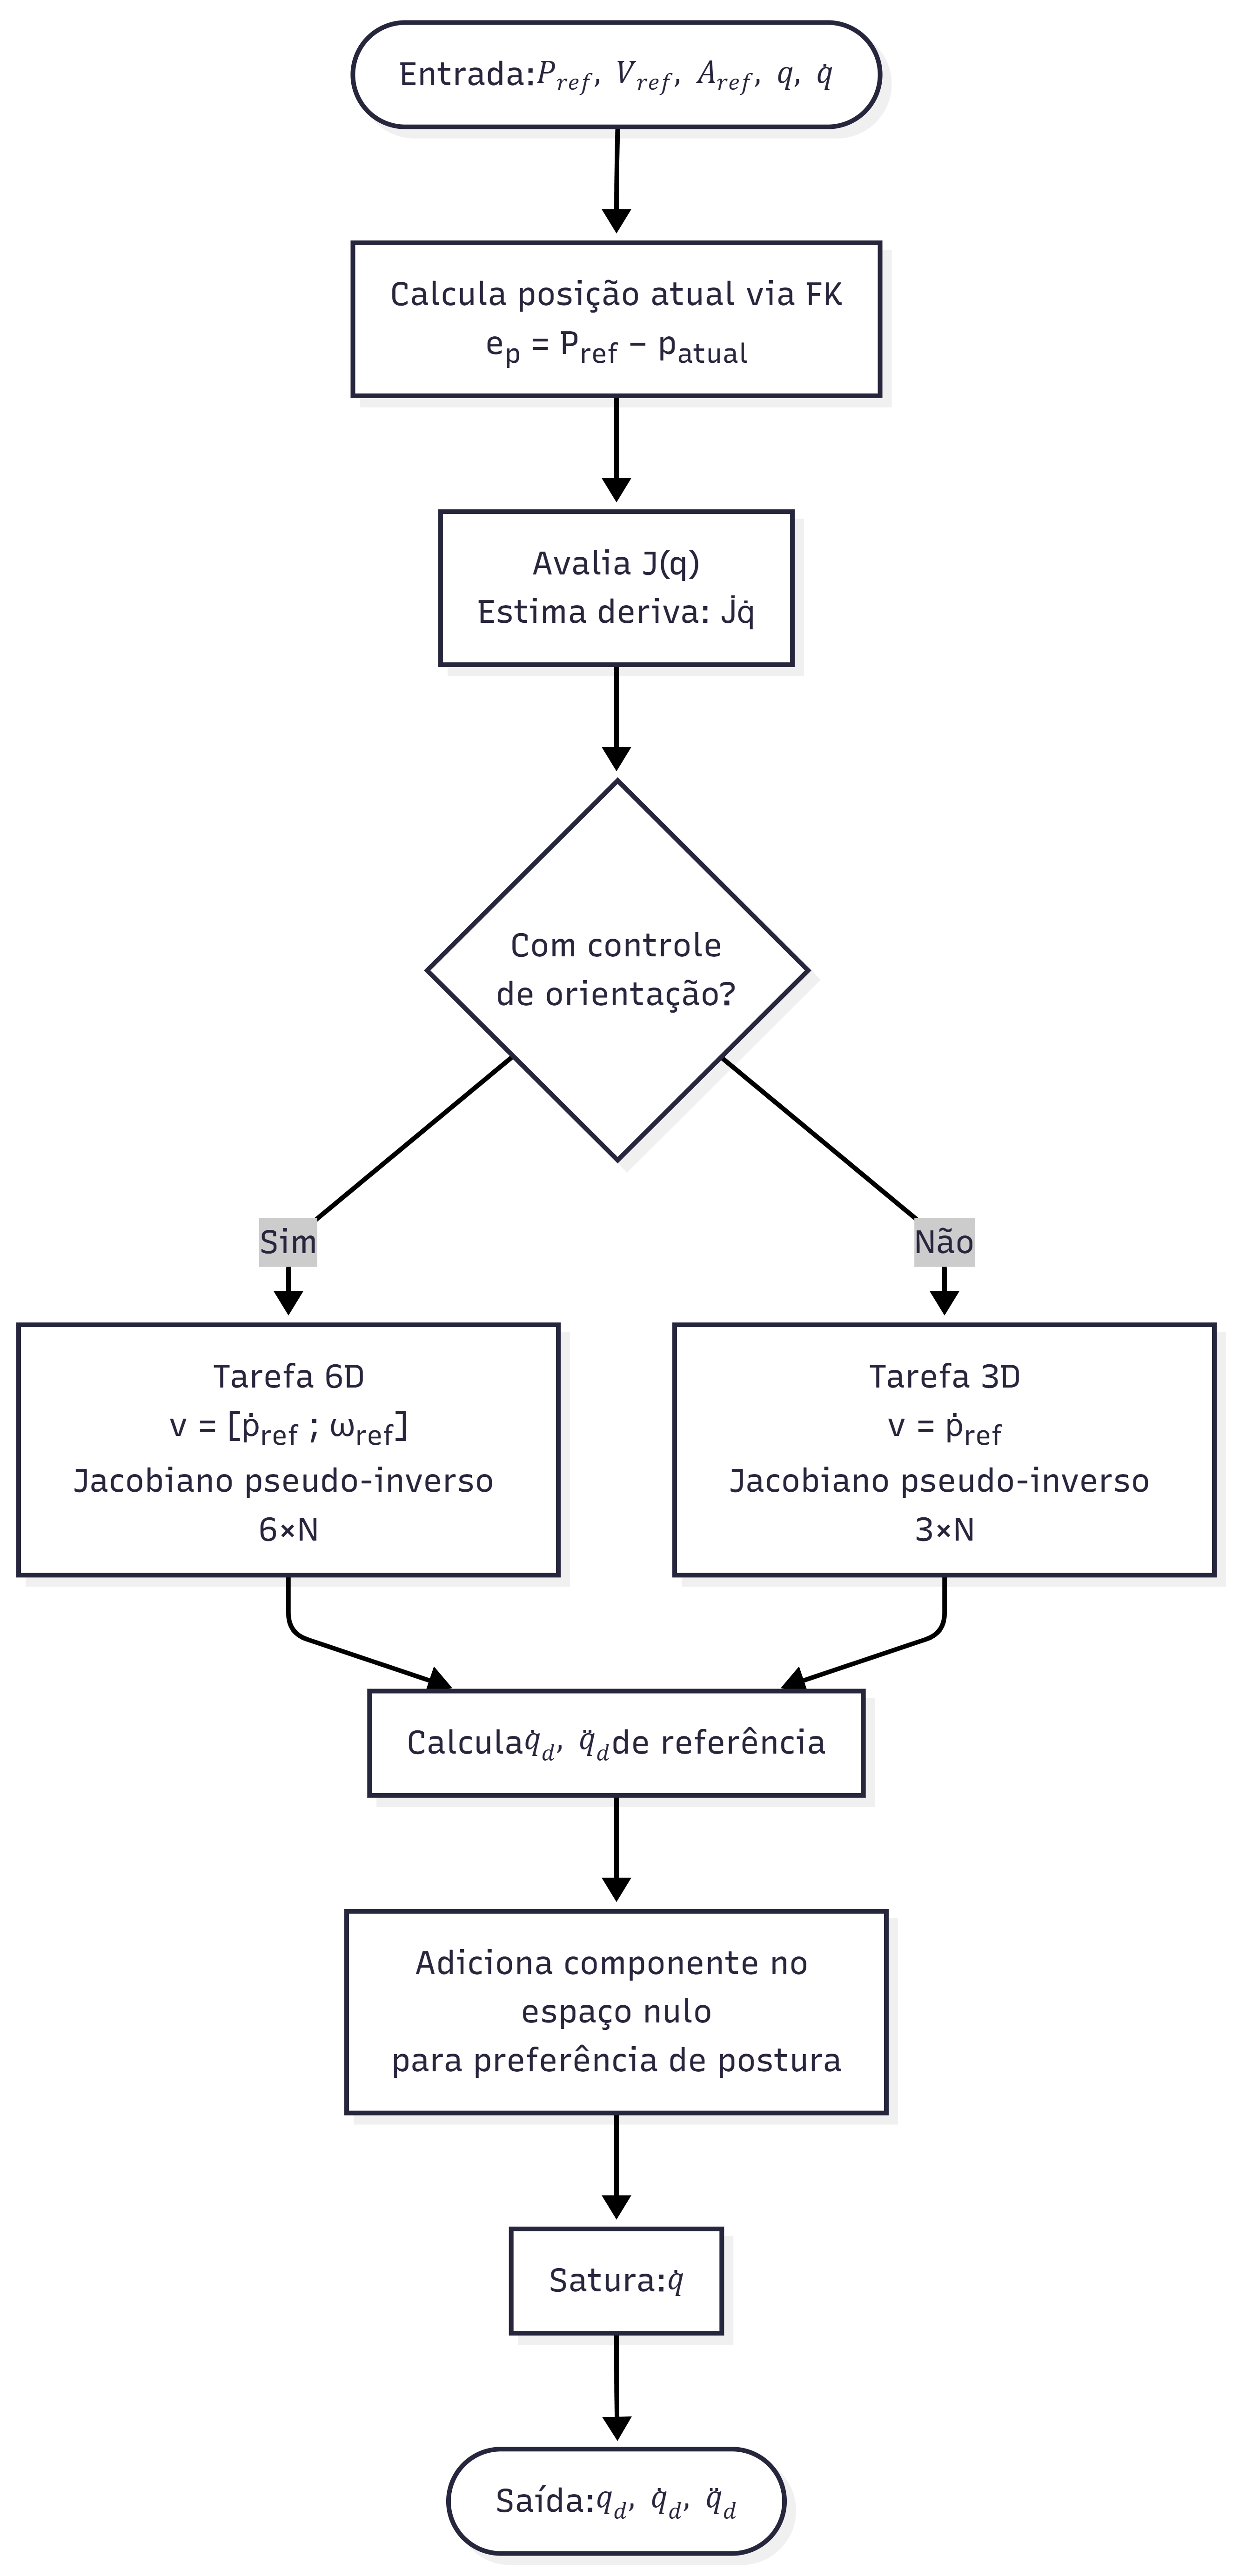
\includegraphics[width=0.7\textwidth]{figuras/Diagramas/Diagrama 6a — CLIK Cinemática Inversa Numérica.png}
    \caption{Fluxo do algoritmo CLIK (\textit{Closed-Loop Inverse Kinematics}) implementado no \textit{Hephaestus}: recebe as referências cartesianas $\{P_{\text{ref}}, \dot{P}_{\text{ref}}, \ddot{P}_{\text{ref}}\}$ e produz as referências de junta $\{q_d, \dot{q}_d, \ddot{q}_d\}$ por pseudo-inversão amortecida DLS (Equação~\eqref{eq:dls_pos}) com gestão de redundância por projeção no espaço nulo \cite{chiaverini1994review, nakamura1986inverse, chiaverini1997singularity}.}
    \label{fig:clik_cinematica}
\end{figure}

% ==============================================================================
\section{Integrador Simplético de Euler com Substeps}
\label{sec:integrador}
% ==============================================================================

\subsection{Hierarquia de Passos de Tempo}

O integrador numérico opera em dois níveis de passo de tempo, independentes entre si:

\begin{itemize}
    \item $\Delta t_{\text{phys}}$: passo de integração física, tipicamente $\Delta t_{\text{phys}} = 10^{-3}$ s. Determina a fidelidade numérica da integração das equações de movimento.
    \item $\Delta t_{\text{vis}}$: passo de amostragem para visualização e armazenamento de resultados, tipicamente $\Delta t_{\text{vis}} = 5 \times 10^{-2}$ s. Determina a taxa de frames da animação.
\end{itemize}

O número de \textit{substeps} por frame de visualização é:
\begin{equation}
    N_s = \left\lceil \frac{\Delta t_{\text{vis}}}{\Delta t_{\text{phys}}} \right\rceil,
    \label{eq:substeps}
\end{equation}
e o $\Delta t_{\text{vis}}$ efetivo é ajustado para $N_s \cdot \Delta t_{\text{phys}}$, garantindo que o passo visual seja um múltiplo inteiro do físico. Essa separação permite aumentar a fidelidade numérica sem custo proporcional de armazenamento ou renderização: para $\Delta t_{\text{vis}} = 0.05$ s e $\Delta t_{\text{phys}} = 10^{-3}$ s, obtêm-se 50 substeps por frame, com apenas um frame armazenado por cada 50 avaliações de dinâmica \cite{leimkuhler2004simulating}.

\subsection{Integrador Simplético de Euler}

A integração das equações de movimento \eqref{eq:motion_equation} (Capítulo~\ref{cap:revisao}) é realizada pelo método de Euler Simplético de primeira ordem. A cada substep físico, a dinâmica direta é resolvida por:
\begin{equation}
    \ddot{q}^n = M^{-1}\!\left(q^n\right)\left[\tau^n_{\text{ctrl}} + \tau^n_{\text{dist}} - C^n - G^n - \tau^n_{\text{pass}}\right],
    \label{eq:dyn_direct}
\end{equation}
onde $\tau^n_{\text{ctrl}}$ é o torque do controlador, $\tau^n_{\text{dist}}$ é o torque de distúrbio externo (opcional), $\tau^n_{\text{pass}}$ reúne as forças passivas (atrito + arrasto, descritos na Seção~\ref{sec:dissipative}), e $C^n$, $G^n$ são avaliados na configuração atual $(q^n, \dot{q}^n)$. A inversão de $M$ é realizada por \texttt{np.linalg.solve}, que utiliza decomposição LU — numericamente mais estável e eficiente que o cálculo explícito da inversa \cite{golub2013matrix}.

A atualização do estado segue a sequência simplética:
\begin{align}
    \dot{q}^{n+1} &= \dot{q}^n + \ddot{q}^n\,\Delta t_{\text{phys}}, \label{eq:symplectic1}\\
    q^{n+1} &= q^n + \dot{q}^{n+1}\,\Delta t_{\text{phys}}. \label{eq:symplectic2}
\end{align}

A ordem em que velocidade e posição são atualizadas — velocidade \emph{antes} da posição — distingue o integrador simplético do Euler explícito padrão. Enquanto o Euler explícito acumula energia seculamente (instabilidade numérica suave), o Euler Simplético preserva uma ``energia modificada'' próxima da hamiltoniana real do sistema, garantindo estabilidade de longo prazo \cite{leimkuhler2004simulating, hairer2006geometric}. Para simulações de controle em malha fechada com duração moderada (tipicamente $< 30$ s), essa diferença é crítica para a fidelidade dos torques calculados e da resposta do controlador.

Após cada atualização, as coordenadas de juntas rotacionais são restritas ao intervalo $(-\pi, \pi]$ pelo operador de envolvimento (\textit{wrap}):
\begin{equation}
    q_i \leftarrow (q_i + \pi) \bmod 2\pi - \pi, \quad \forall i \text{ tal que a junta } i \text{ é rotacional},
    \label{eq:wrap}
\end{equation}
assegurando que os erros de junta $e_i = q_{d,i} - q_i$ representem sempre o menor caminho angular — condição necessária para a estabilidade de controladores com ganho proporcional \cite{spong2020robot}. Uma verificação de finitude (\texttt{np.isfinite}) é aplicada a $q$ e $\dot{q}$ após cada substep; caso valores NaN ou Inf sejam detectados, a simulação é interrompida com uma exceção descritiva, prevenindo propagação silenciosa de instabilidades numéricas.

% ==============================================================================
\section{Estratégias de Controle Não-Linear}
\label{sec:controle_impl}
% ==============================================================================

Quatro estratégias de controle não-linear são implementadas no \textit{Hephaestus}, todas recebendo como entrada as referências de junta $\{q_d, \dot{q}_d, \ddot{q}_d\}$ geradas pelo CLIK e as matrizes dinâmicas avaliadas numericamente. Uma única interface unificada — o parâmetro \texttt{ctrl\_params} do método \texttt{run()} — seleciona e configura o controlador ativo, permitindo a comparação direta das estratégias sob condições idênticas de trajetória, modelo e perturbações.

\subsection{Controle por Torque Computado com PID (CTC-PID)}

O Controle por Torque Computado com PID \cite{craig1989introduction, spong2020robot} é a estratégia padrão do simulador. A lei de controle é:
\begin{equation}
    \tau_{\text{CTC-PID}} = M(q)\left[\ddot{q}_d + K_D\dot{e} + K_P e + K_I \int e\,dt\right] + C(q,\dot{q}) + G(q),
    \label{eq:ctc_pid_impl}
\end{equation}
onde $e = q_d - q$, $K_P = k_p I_N$, $K_D = 2\zeta\sqrt{k_p} I_N$ (criticamente amortecido para $\zeta = 1$) e $K_I = k_i I_N$. O ganho derivativo é derivado automaticamente do proporcional pelo método do polinômio característico de segunda ordem, garantindo amortecimento crítico para qualquer valor de $k_p$ \cite{astrom1995theory}.

O integrador é sujeito a \textit{anti-windup} por clamping:
\begin{equation}
    \int e\,dt \leftarrow \text{clip}\!\left(\int e\,dt + e\,\Delta t,\;  -e_{\max},\; e_{\max}\right),
    \label{eq:antiwindup}
\end{equation}
onde $e_{\max}$ é o limite de \textit{windup} configurável, que previne a acumulação do integrador durante períodos de saturação do atuador \cite{astrom1995theory}. Com modelo dinâmico exato, a lei CTC cancela a não-linearidade e a dinâmica de erro satisfaz $\ddot{e} + K_D\dot{e} + K_P e = 0$, que é um sistema linear estável de segunda ordem \cite{craig1989introduction}.

\subsection{Controle por Modo Deslizante (CT-SMC)}

O Controle por Modo Deslizante \cite{slotine1991applied} define a superfície deslizante:
\begin{equation}
    S = \dot{e} + \lambda e, \qquad e = q - q_d,
    \label{eq:sliding_surface}
\end{equation}
e a lei de controle baseada em modelo:
\begin{equation}
    \tau_{\text{SMC}} = M(q)\left[\ddot{q}_{d,f} - \lambda\dot{e} - K\tanh(S/\phi)\right] + C(q,\dot{q}) + G(q),
    \label{eq:smc_impl}
\end{equation}
onde $\ddot{q}_{d,f} = \alpha\,\ddot{q}_d + (1-\alpha)\,\ddot{q}_{d,f}^{\text{prev}}$ é um filtro passa-baixas da aceleração de referência com coeficiente $\alpha \in (0,1]$. O filtro atenua picos de aceleração oriundos das derivadas do CLIK, que seriam amplificados pelo ganho $\lambda$ na lei de controle — uma instabilidade prática frequentemente não mencionada nas formulações teóricas do CT-SMC \cite{slotine1991applied, edwards1998sliding}.

A função $\tanh(S/\phi)$ substitui o sinal descontínuo $\text{sign}(S)$ pela camada limite de espessura $\phi > 0$, eliminando o \textit{chattering} (oscilações de alta frequência) ao custo de uma robustez assintótica dentro da camada \cite{slotine1991applied}. A análise formal da robustez com camada limite foi conduzida por Burton e Zinober \cite{burton1986continuous}: para perturbações $|d| \leq D$, o erro de regime permanente é limitado por $\|S\|_\infty \leq \phi \cdot D / K$, o que permite ao projetista estabelecer um compromisso explícito entre \textit{chattering} e precisão de rastreamento.

\subsection{Super-Twisting (STA)}

O algoritmo Super-Twisting (STA), proposto por Levant \cite{levant1993sliding}, é um modo deslizante de segunda ordem que elimina o \textit{chattering} intrinsecamente ao produzir um sinal de controle contínuo. A superfície deslizante é idêntica à Equação~\eqref{eq:sliding_surface}, e a parcela de modo deslizante é:
\begin{align}
    v_{\text{sw}} &= -k_1\,|S|^{1/2}\,\text{sign}(S) + z, \label{eq:sta1_impl}\\
    \dot{z} &= -k_2\,\text{sign}(S), \label{eq:sta2_impl}
\end{align}
onde $z$ é uma variável interna integrada numericamente por Euler explícito: $z^{n+1} = z^n - k_2\,\text{sign}(S^n)\,\Delta t$. A lei de controle completa é:
\begin{equation}
    \tau_{\text{STA}} = M(q)\left[\ddot{q}_{d,f} - \lambda\dot{e} + v_{\text{sw}}\right] + C(q,\dot{q}) + G(q).
    \label{eq:sta_ctrl}
\end{equation}

O sinal $v_{\text{sw}}$ é contínuo porque $z$ integra o sinal descontínuo, fazendo $v_{\text{sw}}$ variar continuamente mesmo que $\text{sign}(S)$ seja descontínuo. Moreno e Osorio \cite{moreno2012strict} forneceram uma função de Lyapunov estrita para o STA, estabelecendo condições de ganho suficientes para convergência em tempo finito com distúrbio de derivada limitada $|\dot{d}| \leq \delta$: $k_2 > \delta$ e $k_1 > 2\sqrt{k_2\,\delta}$. A convergência em tempo finito de $S \to 0$ e $\dot{S} \to 0$ diferencia qualitativamente o STA do CT-SMC de primeira ordem, cuja convergência é assintótica \cite{levant1993sliding, utkin2017sliding}.

O filtro de $\ddot{q}_{d,f}$ é compartilhado com a implementação do CT-SMC, sendo parametrizado pelo mesmo coeficiente $\alpha$, o que garante comparabilidade direta das duas estratégias quando $\lambda$, $K$ (CT-SMC) e $k_1$, $k_2$ (STA) são ajustados para desempenhos nominais equivalentes.

\subsection{Controle por Rejeição Ativa de Distúrbios Linear (LADRC)}

O LADRC (Linear Active Disturbance Rejection Control), proposto por Han \cite{han1995class} e formalizado em versão linear por Gao \cite{gao2003scaling}, é implementado de forma descentralizada — um ESO e uma lei de controle por junta, ignorando o acoplamento dinâmico \cite{huang2014active}. Para a junta $i$, a dinâmica nominal é reescrita como:
\begin{equation}
    \ddot{q}_i = b_{0,i}\,\tau_i + f_i, \qquad f_i = \text{distúrbio total},
    \label{eq:adrc_plant_impl}
\end{equation}
onde $b_{0,i} \approx 1/M_{ii}(q_0)$ é estimado automaticamente a partir da diagonal da matriz de inércia na postura inicial, conforme a opção \texttt{auto\_b0} da configuração.

O ESO de terceira ordem (linear) é integrado por Euler explícito a cada passo $\Delta t_{\text{phys}}$:
\begin{align}
    z_1^{n+1} &= z_1^n + \Delta t\left[z_2^n - \beta_1(z_1^n - q_i^n)\right], \label{eq:eso1_impl}\\
    z_2^{n+1} &= z_2^n + \Delta t\left[z_3^n - \beta_2(z_1^n - q_i^n) + b_0 \tau_i^{n-1}\right], \label{eq:eso2_impl}\\
    z_3^{n+1} &= z_3^n - \Delta t\,\beta_3(z_1^n - q_i^n), \label{eq:eso3_impl}
\end{align}
com $\beta_1 = 3\omega_o$, $\beta_2 = 3\omega_o^2$, $\beta_3 = \omega_o^3$ \cite{gao2003scaling}. A frequência $\omega_o$ é automaticamente limitada por $\omega_o \leq \omega_{\max}/\Delta t$ para garantir estabilidade numérica do ESO discreto: a condição $\omega_o \Delta t \leq 0.1$ é aplicada como heurística de projeto \cite{zheng2010practical}.

A estimativa $z_3^n$ do distúrbio total é suavizada por um filtro IIR de primeira ordem antes de ser usada na lei de controle:
\begin{equation}
    z_3^{\text{filt},n} = \alpha_{\text{filt}}\,z_3^n + (1 - \alpha_{\text{filt}})\,z_3^{\text{filt},n-1},
    \label{eq:z3_filter}
\end{equation}
onde $\alpha_{\text{filt}} \in (0, 1]$ é o coeficiente do filtro ($\alpha = 1$ desativa o filtro). Este filtro é necessário em prática para atenuar o conteúdo de alta frequência que o ESO amplifica nos ciclos iniciais, antes de convergir ao valor real de $f_i$ \cite{han2009pid}.

A lei de controle cancela o distúrbio estimado e acrescenta \textit{feedforward} explícito de $G$ e $C$ para reduzir o distúrbio residual que o ESO precisa estimar:
\begin{equation}
    \tau_i^{\text{LADRC}} = \frac{u_{0,i} - z_{3,i}^{\text{filt}}}{b_{0,i}} + G_i + C_i,
    \label{eq:ladrc_ctrl}
\end{equation}
\begin{equation}
    u_{0,i} = \ddot{q}_{d,i} + k_{p,i}(q_{d,i} - q_i) + k_{d,i}(\dot{q}_{d,i} - \dot{q}_i).
    \label{eq:ladrc_u0}
\end{equation}

O \textit{feedforward} de $G$ e $C$ é especialmente crítico em manipuladores terrestres (onde $G \neq 0$) e no início de trajetórias rápidas (onde $C \propto \dot{q}^2$ cresce rapidamente): sem esses termos, o ESO deve perseguir um distúrbio crescente com lag dinâmico, introduzindo um transiente oscilatório nos primeiros instantes da trajetória. A inclusão do feedforward reduz o distúrbio residual a apenas erros de modelo e perturbações externas — sinais pequenos e quase constantes que o ESO estima com precisão \cite{han2009pid}. A análise de estabilidade do LADRC com esta formulação foi formalizada por Zheng e Gao \cite{zheng2010practical}.

% ==============================================================================
\section{Modelos de Forças Dissipativas}
\label{sec:dissipative}
% ==============================================================================

\subsection{Atrito nas Juntas}

O modelo de atrito nas juntas combina os componentes de Coulomb (atrito estático/cinético) e viscoso (proporcional à velocidade):
\begin{equation}
    \tau_{\text{fric},i} = F_{c,i}\,\tanh\!\left(\frac{\dot{q}_i}{\varepsilon}\right) + B_{v,i}\,\dot{q}_i,
    \label{eq:friction}
\end{equation}
onde $F_{c,i} \geq 0$ é o coeficiente de atrito de Coulomb por junta, $B_{v,i} \geq 0$ é o coeficiente viscoso e $\varepsilon > 0$ é a zona suave (\textit{regularization zone}). O uso de $\tanh$ em vez de $\text{sign}(\dot{q})$ é essencial para evitar descontinuidades que causariam instabilidade numérica no integrador: para $|\dot{q}_i| \gg \varepsilon$, $\tanh(\dot{q}_i/\varepsilon) \approx \text{sign}(\dot{q}_i)$, recuperando o comportamento de Coulomb clássico; para $|\dot{q}_i| \approx 0$, a transição é suave e impede o fenômeno de \textit{stiction} numérico \cite{slotine1991applied}. O valor padrão $\varepsilon = 0.05$ rad/s é calibrado para suavizar sem mascarar a zona de atrito estático em velocidades de junta típicas de manipuladores de laboratório.

\subsection{Arrasto Hidrodinâmico}

No modo \textit{Hydro}, um modelo simplificado de arrasto no espaço de juntas é aplicado como força passiva \cite{fossen2011handbook, antonelli2014modelling}:
\begin{equation}
    \tau_{\text{drag},i} = D_{\text{lin},i}\,\dot{q}_i + D_{\text{quad},i}\,|\dot{q}_i|\,\dot{q}_i,
    \label{eq:drag_impl}
\end{equation}
onde $D_{\text{lin},i}$ e $D_{\text{quad},i}$ são os coeficientes de arrasto linear e quadrático da junta $i$. Esta formulação é equivalente à Equação~\eqref{eq:drag} do Capítulo~\ref{cap:revisao}, parametrizada no espaço de juntas em vez do espaço cartesiano para compatibilidade com o integrador \cite{antonelli2014modelling}. O arrasto quadrático captura os efeitos de pressão (regime turbulento, número de Reynolds elevado) que dominam em velocidades de junta mais altas, enquanto o linear captura o arrasto viscoso do escoamento laminar em baixas velocidades \cite{fossen2011handbook, newman1977marine}.

Ambas as forças dissipativas são aplicadas na equação de dinâmica direta como torques passivos externos:
\begin{equation}
    \ddot{q}^n = M^{-1}\!\left(\tau_{\text{ctrl}}^n - C^n - G^n - \tau_{\text{fric}}^n - \tau_{\text{drag}}^n\right),
    \label{eq:dyn_complete}
\end{equation}
fora do laço do controlador. Essa separação é fisicamente correta: os torques dissipativos são forças do ambiente (não cancelas pelo controlador a priori) e devem ser observados ou estimados para serem compensados — papel que o ESO do LADRC desempenha implicitamente \cite{han2009pid, huang2014active}.

% ==============================================================================
\section{Paralelismo na Avaliação Numérica}
\label{sec:parallel_sim}
% ==============================================================================

A avaliação numérica das funções $f_M$, $f_C$ e $f_G$ a cada passo de integração é o principal gargalo de tempo de execução para sistemas com $N \geq 5$ GDL, onde as expressões compiladas possuem centenas de operações trigonométricas e matriciais. Para mitigar esse custo, o \textit{Hephaestus} suporta avaliação paralela via um executor persistente de processos.

O executor \texttt{ProcessPoolExecutor} é inicializado uma única vez após a compilação (método \texttt{warm\_up\_workers()}), com cada \textit{worker} executando o inicializador \texttt{\_init\_worker} que compila localmente as três funções via \texttt{lambdify} e as armazena no dicionário de módulo \texttt{\_WORKER\_FUNCS}. A cada passo físico, três tarefas são submetidas em paralelo:
\begin{equation}
    \texttt{futures} = \left\{
        M: \texttt{executor.submit}(\texttt{\_eval\_worker}, (\text{"M"}, \textbf{args})), \;
        C: \texttt{executor.submit}(\ldots), \;
        G: \texttt{executor.submit}(\ldots)
    \right\},
    \label{eq:parallel_submit}
\end{equation}
e os resultados são coletados por \texttt{Future.result()} após o despacho das três tarefas, aproveitando a sobreposição de computação \cite{beazley2010understanding}.

A chave da eficiência é a \textbf{persistência} do executor: ao contrário de uma implementação ingênua que instancia e destrói um \textit{pool} por simulação (custo de 2--8 s por instância, conforme medido nos testes), o executor é instanciado uma única vez e reutilizado em todas as chamadas subsequentes a \texttt{run()}. A detecção de mudança no número de \textit{workers} solicita reinicialização automática do executor, garantindo flexibilidade sem custo desnecessário \cite{leu1986automated}.

Quando o paralelismo não está habilitado (\texttt{use\_parallel=False}), as três funções são avaliadas sequencialmente na thread principal — comportamento padrão seguro para executáveis PyInstaller, máquinas com um único núcleo ou ambientes de depuração. Esta opção também é preferida para sistemas com $N \leq 4$ GDL, onde o \textit{overhead} de IPC supera o ganho de paralelismo \cite{beazley2010understanding}.

% ==============================================================================
\section{Verificação de Estabilidade Numérica}
\label{sec:estabilidade_num}
% ==============================================================================

A estabilidade numérica do integrador simplético é governada pela relação entre o passo de integração $\Delta t_{\text{phys}}$ e as frequências naturais do sistema em malha fechada. Para o CTC, a dinâmica de erro é linear de segunda ordem com frequência natural $\omega_n = \sqrt{k_p}$; a condição de estabilidade de Euler simplético exige \cite{leimkuhler2004simulating}:
\begin{equation}
    \Delta t_{\text{phys}} < \frac{2}{\omega_n} = \frac{2}{\sqrt{k_p}},
    \label{eq:stability_condition}
\end{equation}
ou seja, ao menos dois passos por período de oscilação de malha fechada. Para $k_p = 100$ rad$^2$/s$^2$ (ganho típico), $\omega_n = 10$ rad/s e $\Delta t_{\text{phys}} < 0.2$ s — condição satisfeita com folga para $\Delta t_{\text{phys}} = 10^{-3}$ s \cite{hairer2006geometric}. Avisos automáticos são emitidos quando $\Delta t_{\text{phys}} > 10^{-2}$ s ou $\Delta t_{\text{vis}} > 0.1$ s, alertando o usuário sobre potencial instabilidade.

Para o LADRC, a condição adicional de estabilidade do ESO discreto é $\omega_o \Delta t_{\text{phys}} \leq 0.1$, correspondente à frequência de observador máxima $\omega_o^{\max} = 0.1/\Delta t_{\text{phys}} = 100$ rad/s para $\Delta t_{\text{phys}} = 10^{-3}$ s. Este limite é imposto automaticamente pela verificação \texttt{max\_wo\_dt} no construtor do LADRC \cite{zheng2010practical}.

% ==============================================================================
\section{Síntese do Capítulo}
% ==============================================================================

Este capítulo descreveu a arquitetura completa de simulação numérica do \textit{Hephaestus}. O fluxo de execução do método \texttt{run()} integra, em uma única interface unificada, as seguintes contribuições:

\begin{itemize}
    \item \textbf{Planejamento de trajetória} com polinômio cúbico, suportando segmentos lineares e arcos circulares com aceleração \textit{feedforward} analítica e seis modos de referência de orientação, incluindo SLERP geodésico \cite{shoemake1985animating} e controle tangencial.
    \item \textbf{Inicialização robusta} por Levenberg-Marquardt com busca em linha adaptativa \cite{marquardt1963algorithm, armijo1966minimization}, garantindo partida a partir de qualquer configuração factível.
    \item \textbf{CLIK estendido ao espaço 6D}, com \textit{feedforward} de velocidade e aceleração, correção de deriva do Jacobiano, tratamento de singularidades por DLS \cite{nakamura1986inverse} e gestão de redundância via espaço nulo \cite{chiaverini1997singularity, liegeois1977automatic}.
    \item \textbf{Integrador simplético de Euler} com \textit{substeps} independentes da taxa de visualização, garantindo estabilidade de energia a longo prazo e alta fidelidade numérica \cite{leimkuhler2004simulating, hairer2006geometric}.
    \item \textbf{Quatro controladores não-lineares} comparáveis: CTC-PID \cite{craig1989introduction, astrom1995theory}, CT-SMC com camada limite \cite{slotine1991applied, burton1986continuous}, Super-Twisting STA com convergência em tempo finito \cite{levant1993sliding, moreno2012strict} e LADRC descentralizado com ESO de terceira ordem \cite{gao2003scaling, zheng2010practical, huang2014active}.
    \item \textbf{Forças dissipativas} de atrito nas juntas (Coulomb + viscoso, suavizado por $\tanh$) e arrasto hidrodinâmico (linear + quadrático) \cite{fossen2011handbook, antonelli2014modelling}, aplicadas separadamente do controle para máxima fidelidade física.
    \item \textbf{Executor paralelo persistente} para avaliação paralela de $M$, $C$, $G$ a cada substep, com custo de \textit{spawn} amortizado sobre toda a simulação \cite{beazley2010understanding, leu1986automated}.
\end{itemize}

O Capítulo seguinte apresenta os resultados experimentais obtidos com a plataforma \textit{Hephaestus} em dois cenários de validação: um manipulador serial de 3 GDL em ambiente terrestre e um UVMS de 6 GDL em ambiente subaquático, comparando as quatro estratégias de controle em termos de erro de rastreamento, torques requeridos e resposta a perturbações externas.
